% fig2: science prism, oblique schematic, solid + 2 dashed (AC bottom, A1C long)
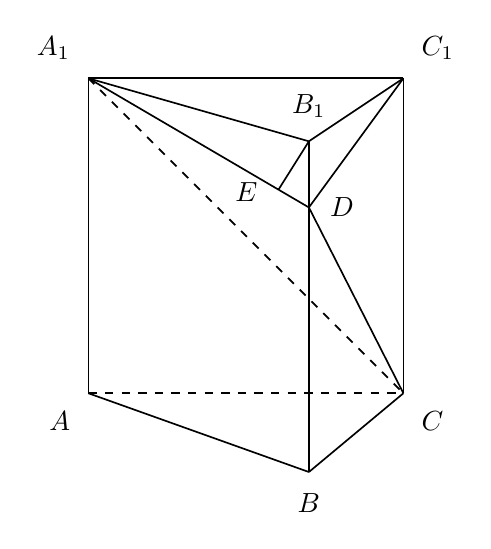
\begin{tikzpicture}[x=1cm,y=1cm,line width=0.6pt,font=\normalsize]
\coordinate (A1) at (0,5);
\coordinate (C1) at (4,5);
\coordinate (B1) at (2.8,4.2);
\coordinate (A) at (0,1);
\coordinate (C) at (4,1);
\coordinate (B) at (2.8,0);
\coordinate (D) at (2.8,3.36);
\coordinate (E) at (2.413793,3.586207);
% outer prism solid
\draw (A1) -- (C1);
\draw (A1) -- (A);
\draw (C1) -- (C);
\draw (B1) -- (B);
\draw (A) -- (B);
\draw (B) -- (C);
% top face
\draw (A1) -- (B1);
\draw (C1) -- (B1);
% interior solid
\draw (A1) -- (D);
\draw (B1) -- (E);
\draw (C1) -- (D);
\draw (D) -- (C);
% hidden dashed
\draw[dashed] (A) -- (C);
\draw[dashed] (A1) -- (C);
% labels offset to avoid strokes
\node[above left,xshift=-3pt,yshift=3pt] at (A1) {$A_{1}$};
\node[above right,xshift=3pt,yshift=3pt] at (C1) {$C_{1}$};
\node[above,xshift=0pt,yshift=5pt] at (B1) {$B_{1}$};
\node[below left,xshift=-3pt,yshift=-3pt] at (A) {$A$};
\node[below right,xshift=3pt,yshift=-3pt] at (C) {$C$};
\node[below,xshift=0pt,yshift=-4pt] at (B) {$B$};
\node[right,xshift=4pt,yshift=0pt] at (D) {$D$};
\node[left,xshift=-4pt,yshift=-1pt] at (E) {$E$};
\end{tikzpicture}
